\documentclass{article}
\usepackage{graphicx}

\title{Lecture Notes for Computer Networks 21/9/18}
\author{Divij Singh}
\date{21/09/18}


\begin{document}

	\maketitle
	For this class, we are looking at communciation between two specific nodes, A and B. They are part of a network of several nodes, and are conencted via a physical medium, such as radio waves or physical cables.\\

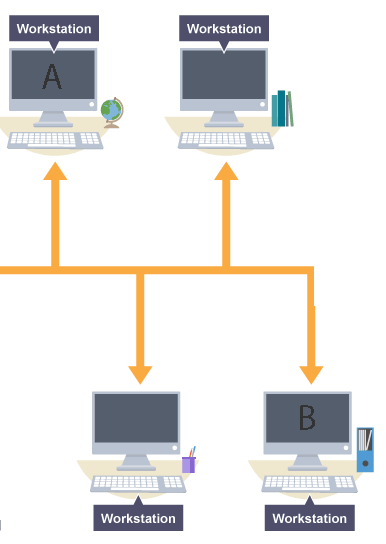
\includegraphics[scale=0.5]{scribe_diagram_1.png}\\

The concern is that when we send a message from A to B, other nodes may be sending a message on the same network. If these messages collide, there will be a loss of information.\\
\\
Thus, we require something to coordinate this exchange of information. We call such mechanisms protocols. The problem is the Medium Access Problem, which is addressed by Medium Access Protocols (MACs).\\
\\
We require a decentralised solution, because if we use a Master Node for coordination, we run the risk of the entire network going down if the Master Node does.\\
\\
There are three broad protocol approaches for solving the problem, used in Ethernet/LAN connections:\\
\begin{itemize}
\item Channel Partitioning Protocol
\item Randem Access Protocol (The Most Important approach)
\item Turn Taking Protocol
\end{itemize}

Of Random Access Protocol, there are three methods we will examine.\\
\begin{itemize}
\item Slotted ALOHA
\item Pure Aloha
\item CSMA/CD (Carrier Sense Multiple Access Collision Detection, used in ethernet)
\end{itemize}
The Slotted ALOHA methoid:\\
This is a hypothetical protocol. It works with the structure of one Master Node, which has unique activity, and several smaller nodes. We shall have these nodes range from $n_1$ to $n_i$.\\
The network's time begins at $t_0$, after which it has regular intervals of time $t$. The protocol states that every time a node has a frame to transmit, it waits for the next time interval, and at that time it begins transmitting the message.\\
The time sync between nodes is ensured by the Master Node, and the time slots are enough for a node to transmit the frame, for it to physically travel, and for it to be received by the other nodes.\\
Every nodes sends frames of equal size, say, $L$ bits. So if the network has a bandwith of $M$ bits per second, it should be sufficient to send $L$ bits in the time $t$.\\
Now, the issue of collision. Say node $n_1$ sends a message at the same time as node $n_3$. This would result in a collision. Under the protocol, once this collision is detected(via hardware), the nodes will realise they must re-transmit.\\
So, according to a probability P, they will decide whether or not to re-transmit at the next time interval ($t_0 + t$). This results in either:
\begin{itemize}
\item Both nodes sending the message
\item One node sending a message
\item Neither node sending a message
\end{itemize}
At the time slot following this ($t_0 +t+t$), if the node has not send the message in time slot $t_0 + 1$, it will immediately attempt to transmit the message again. Should there be another collision, the process repeates.\\
The probability of a succesful transmission in one slot (that is there are no collisions and no silences) is determined by $P[Success] = P[n_1 \land \bar{n_2} \land \bar{n_3} ...] + P[\bar{n_1} \land n_2 \land \bar{n_3} ...] + ... = nP(1-P)^{n-1}$\\
In order to maximise the probability, we can use the following formula:\\
$\theta(P) =nP(1-P)^{n-1}$\\
$Log \theta(P)=log n+ log P + (n-1)log (1-P)$\\
$\frac{d(log\theta(P))}{dP} = 0+\frac{1}{P}+\frac{n-1}{1-P}-\frac{1}{P}-\frac{n-1}{1-P}$\\
\\
$\frac{d(log\theta(P))}{dP} = 0$\\
\\
$\frac{1}{P} - \frac{n-1}{1-P} = 0$\\
$P = \frac{1}{P}$\\
Thus we get the highest effeciency when we set $P$ as $\frac{1}{n}$\\
The optimum efficiency of ALOHA as number of nodes approaches infinity is equal to $\frac{1}{e} = 0.37$
\\
\\
\\
\\
\section{Background of ALOHA protocol}
ALOHA was the project name for one of the first networks. Designed as a radio network, it was developed at the University of Hawaii by Norman Abramson.\\
It consisted of a primary host at the University, with several smaller nodes around the various islands of Hawaii. The primary node would operate on one frequency, and it would broadcast a message to the other stations. The others would then reply on a separate frequency.\\
The issue arose of the waves interfereing with each other when the stations attempted to reply, which led to the estblishment of the Pure ALOHA protocol.

\end{document}